\documentclass{article}
\usepackage[utf8]{inputenc}
\usepackage[a4paper, total={6in, 8in}]{geometry}
\usepackage{natbib}
\usepackage{graphicx}
\usepackage{fancyhdr}
\usepackage{caption}
\usepackage{subcaption}
\usepackage{float}
\fancyhf{}
\fancyhead[L]{
\includegraphics[width=0.25\textwidth,height=10.0mm]{logo}}
\setlength{\headheight}{5.50mm}
\pagestyle{fancy}
\renewcommand{\headrulewidth}{0pt}

\title{ EE463 Static Power Conversion \\AC to DC Motor Drive Project}
\author{Ozan Can İYİER\\Samet YILDIRIM\\Furkan KARACABEY }
\date{January 2019}



\begin{document}
\maketitle

\begin{figure}[h!]
\centering

\includegraphics[scale=1]{logo.png}
\label{fig:members}
\end{figure}
\newpage
\tableofcontents
\newpage
\section{Introduction}

As Static Power Conversion Course project, we are assigned to design an AC to DC Motor Driver which can drive a specified DC motor under full load by controlling the speed. AC input of the system is supplied by a auto-transformer (i.e variac). By using the variac this way, we forced it to act as a fixed transformer. Hence, our product will be able to used industrial purposes.
\par Power electronics is an area which combines high and low voltages. In our project, we deal with both high and low voltages. By designing our circuit, the most challenging part was controlling the IGBT, because we fed the gate of IGBT with Arduino which drives currents in millimetre level. Unlike control part, we drive the rest of the circuit in 10-20 Ampere levels. In order to protect our Arduino, we used some protection circuits. In addition, the other problem that we faced during design process is over-heating. Because the circuit operates under high voltage and current conditions. All components were on the border of the over-heating. Hence, we added some extra components to prevent over-heating.
\par During design process, we considered all of the problems and other possible problems that we can face during test. This reports includes related information about problem statement, possible solution approaches, design specifications, simulation,test and demonstration results. 

\section{Project Description}
In this project, FOSFOS AG is assigned to drive a Crompton Parkinson DC Motor which is indicated at figure 1. 
\begin{figure}[h!]
\centering
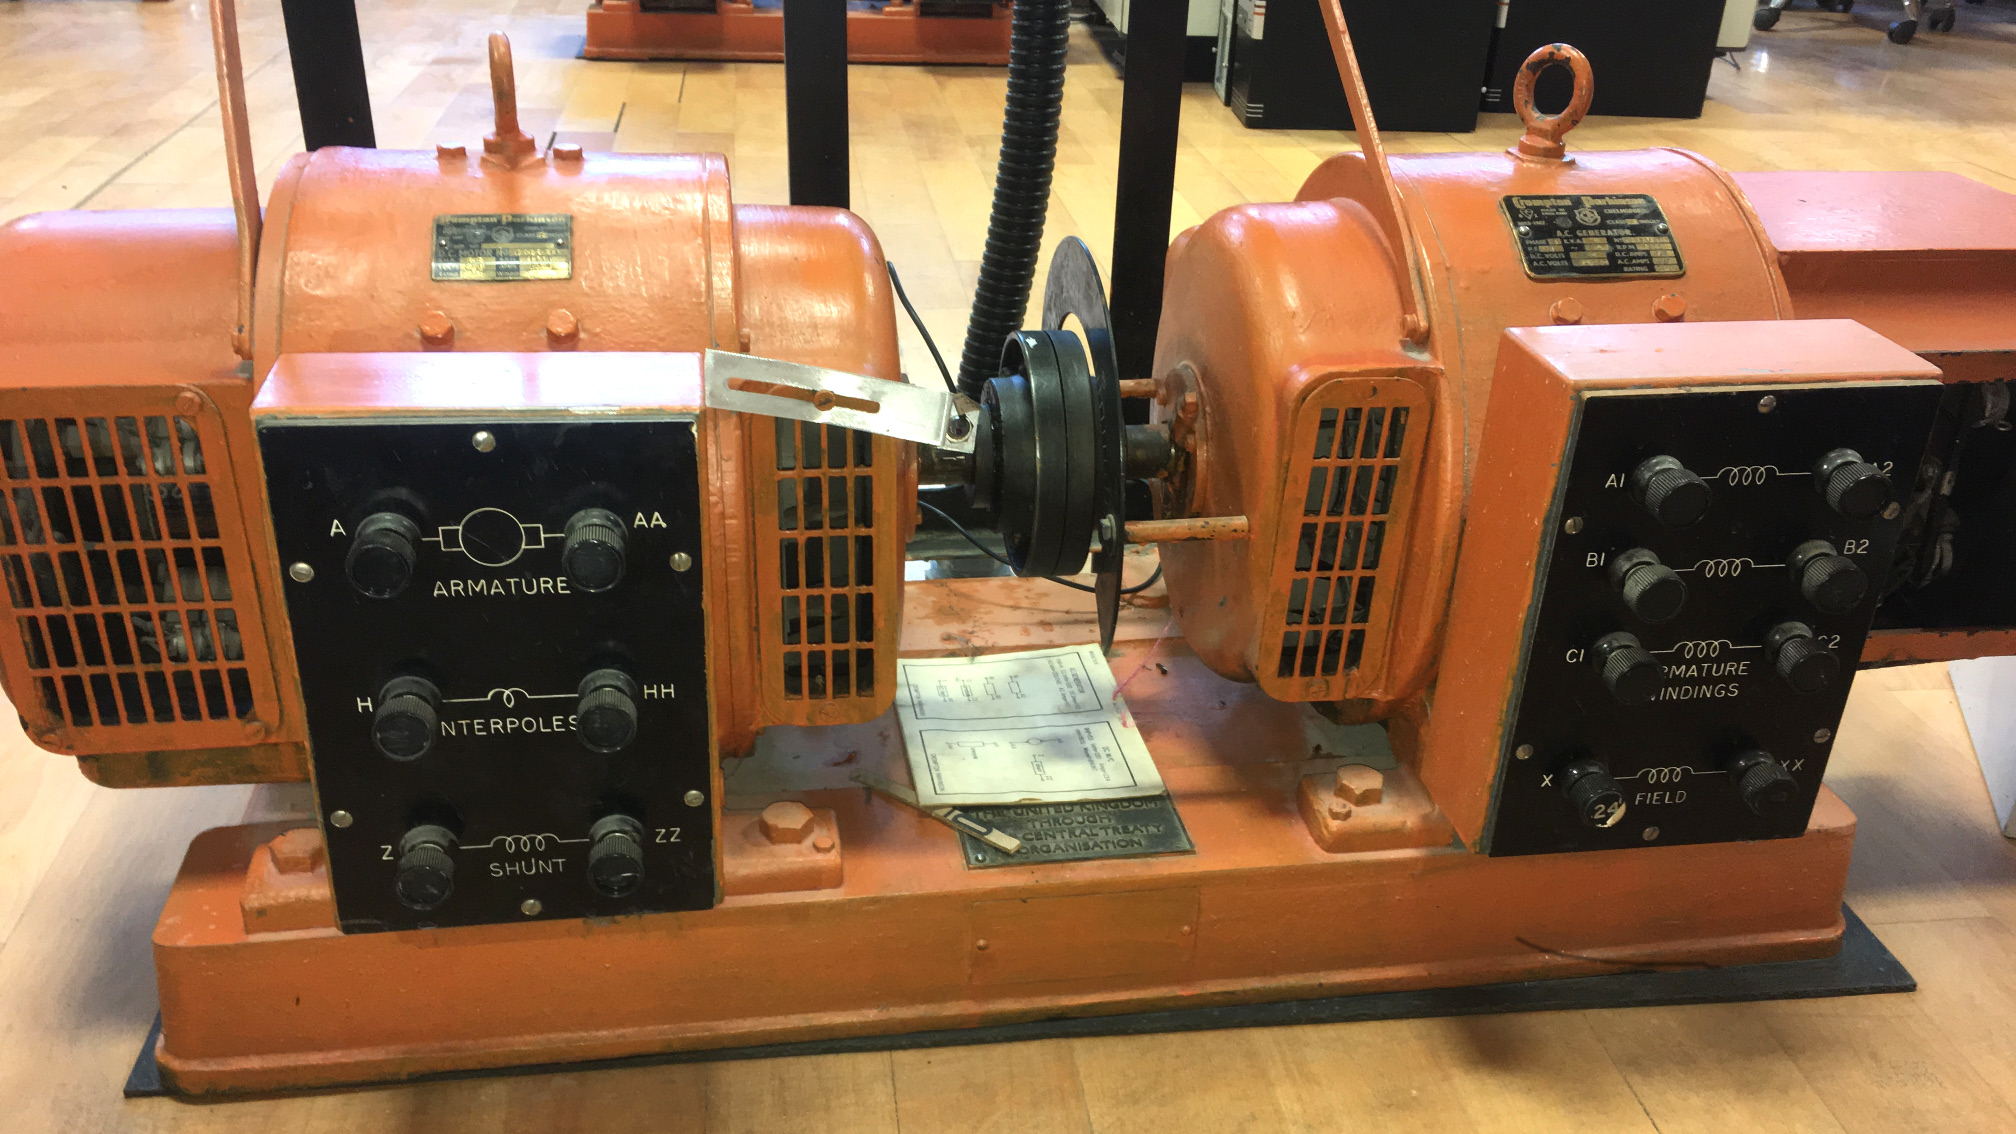
\includegraphics[scale=0.10]{motorsetup}
\caption{Crompton Parkinson DC Motor }
\label{fig:members}
\end{figure} 

The ratings of the DC Motor is indicated at following table;\\
\noindent Table 1: The Specifications of DC Motor
\begin{figure}[h!]
\centering
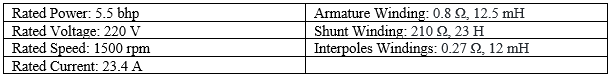
\includegraphics[scale=0.8]{motordetay}
\label{fig:members}
\end{figure} 

The input of the project is specified as three or single phase AC grid supplied by variac. The output voltage of the design should be higher than 180Vdc. In addition to these features, the system should (9)control the speed of motor. Heating and isolation conditions of the system also should be sufficient for long term usages. 

\subsection{Solution Approaches}%Furkan
This project has three main topologies to control-drive DC motor. These are three-phase thyristor rectifier, one-phase thyristor rectifier and three-phase diode rectifier with a buck converter. This part of the report includes comparison of these topologies with advantages and disadvantages, simulations of them. Simulations are done by Simulink software. Simulations provide just an example of these topologies with loads.
\subsubsection{Three-Phase Thyristor Rectifier} %Furkan
This topology which can be seen in figure 2 below includes 6 thyristors. Thyristors must be opened by different gate signals so a fixed delay between the gates is required for switching signals. These gate signals are also used to control DC output. 
\begin{figure}[h!]
\centering
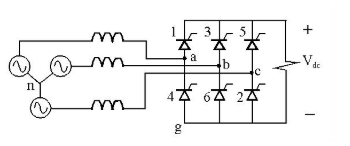
\includegraphics[scale=0.65]{ucfazthytopo}
\caption{Three-Phase Thyristor Rectifier}
\label{fig:members}
\end{figure} 
\par To analyze this topology FosFos AG created a design example on Simulink. This design includes a R load and thyristors have 30-degree firing angle. Figure 3 and 4 shows the schematic of the three-phase thyristor rectifier and output voltage waveform of it.
\begin{figure}[h!]
\centering
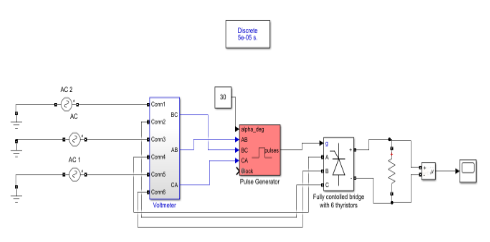
\includegraphics[scale=0.55]{ucfazthycct}
\caption{Simulink Schematic of the Three-Phase Thyristor Rectifier}
\label{fig:members}
\end{figure} 

\begin{figure}[h!]
\centering
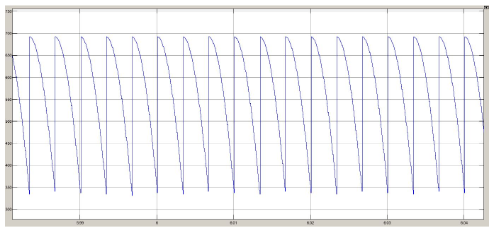
\includegraphics[scale=0.55]{ucfazthyvoltage}
\caption{Output Voltage Waveform of the Three-Phase Thyristor Rectifier}
\label{fig:members}
\end{figure} 

\subsubsection{One-Phase Thyristor Rectifier}%Furkan
This topology which can be seen in figure 5 below includes 4 thyristors. DC output voltage can be controlled by using two thyristors per half-cycle. Q1-Q4 and Q2-Q3 thyristors are firing together for positive and negative cycle.  
\begin{figure}[h!]
\centering
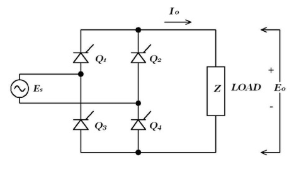
\includegraphics[scale=0.55]{birfazthytopo}
\caption{One-Phase Thyristor Rectifier}
\label{fig:members}
\end{figure} 
\par Simulink analysis of this topology which is shown in figure 6 was done with R-L Load and the output voltage which includes comparison of input and output can be seen in figure 7.

\begin{figure}[h!]
\centering
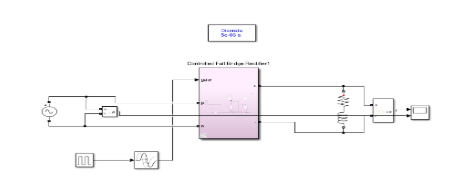
\includegraphics[scale=0.75]{birfazthycct}
\caption{Simulink Schematic of the One-Phase Thyristor Rectifier}
\label{fig:members}
\end{figure} 

\begin{figure}[h!]
\centering
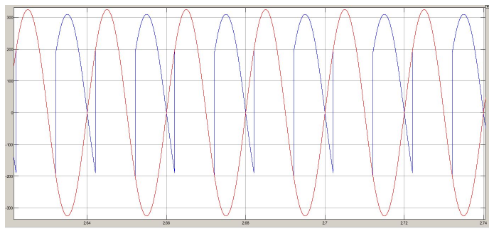
\includegraphics[scale=0.55]{birfazthyvoltage}
\caption{Input-Output Voltage Waveform of the One-Phase Thyristor Rectifier}
\label{fig:members}
\end{figure} 


\subsubsection{Three-Phase Diode Rectifier \& Buck Converter}%Furkan
This topology which can be seen in figure 8 below includes 6 diodes; a switch element which can be Mosfet, IGBT i.e; a freewheeling diode which is conducted when the switch is off; and a LC filter which is used for getting smooth output voltage. Output DC voltage cannot be controlled by bridge rectifier, but it can be controlled by driving switch element’s gate.
\begin{figure}[h!]
\centering
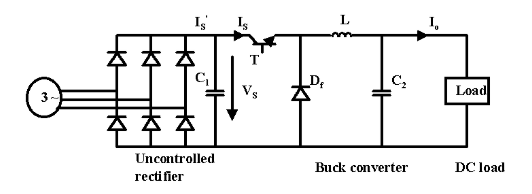
\includegraphics[scale=0.7]{ucfazdiodetopo}
\caption{Three-Phase Diode Rectifier with Buck Converter}
\label{fig:members}
\end{figure} 

\par Simulation of this topology was done with two filters which are DC Link capacitor and LC filter and an R-L Load. Duty Cycle was selected \%45 and the switching frequency was 7800kHz. The schematic of the simulation and graph of the output voltage waveform are shown in figure 9 and 10.
\begin{figure}[h!]
\centering
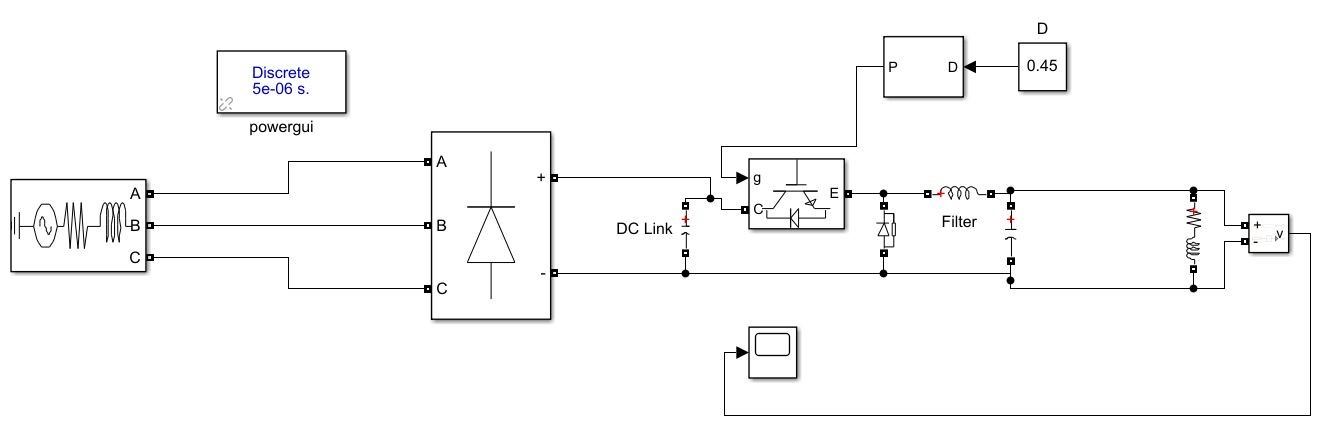
\includegraphics[scale=0.3]{furkancct}
\caption{Simulink Schematic of the Three-Phase Diode Rectifier with Buck Converter}
\label{fig:members}
\end{figure}


\begin{figure}[h!]
\centering
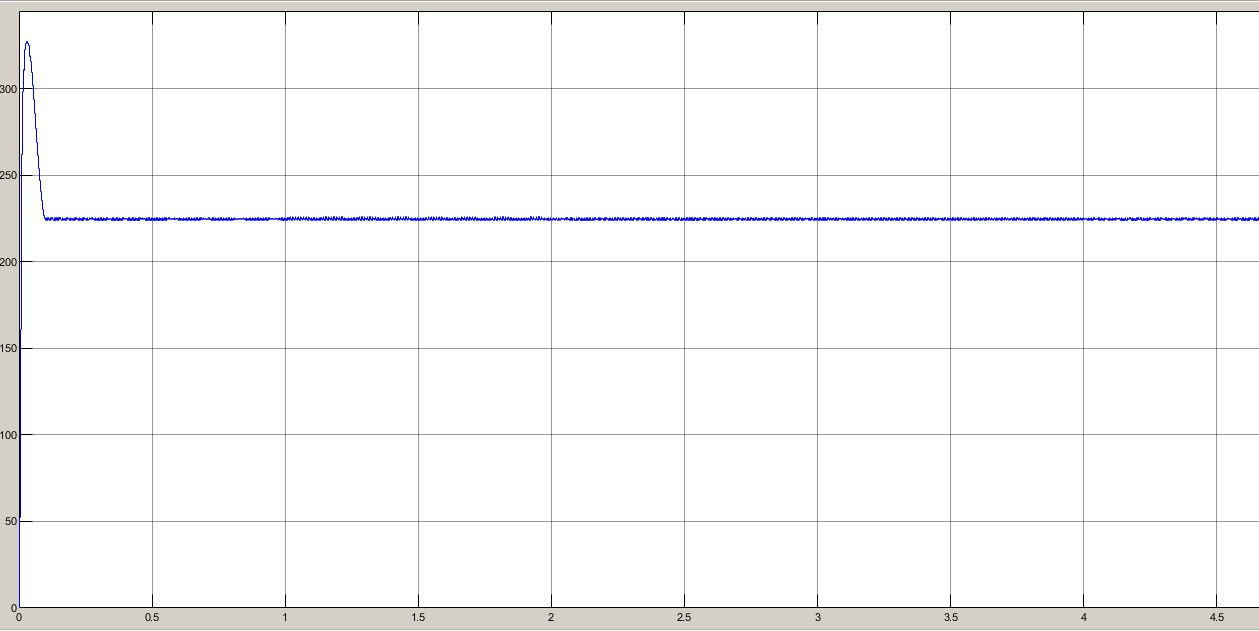
\includegraphics[scale=0.25]{furkanvoltage}
\caption{Output Voltage Waveform of the Three-Phase Diode Rectifier with Buck Converter}
\label{fig:members}
\end{figure}

\newpage
\subsection{Comparison of Solution Approaches} %furkan

\noindent Table 2:Advantages and Disadvantages of Solution Approaches
\begin{figure}[h!]
\centering
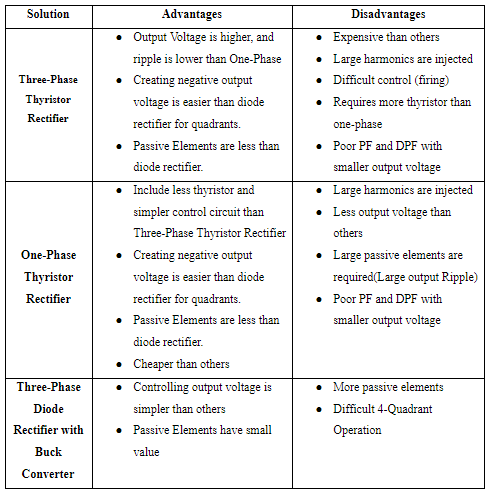
\includegraphics[scale=0.8]{comporison}
\label{fig:members}
\end{figure}
\section{Design Specifications}%Furkan
FosFos AG plans to design cheaper and efficient project for driving DC Motor. Project design of FosFos AG includes a three-phase diode rectifier, a DC link capacitor which is used for filtering the rectifier output, a switch element and a freewheeling diode.In addition to these parts, some modifications are applied to prevent possible issues.For example, LC filter of the output of the buck converter is not included because motor can be considered not only a load but also a filter. The other example of this is in order to prevent over-heating issues power diode and IGBT is connected to a heatsink. The other modification applied is inserting a snubber circuit to prevent overshoot voltages occuring between collector and emittor. To control gate of the switch element, Arduino Nano is selected because it is enough to give switching frequency and size of the component is very suitable for simple design.
\par Reasons of the rectifier selection can be seen below.
\begin{itemize}
\item FosFos AG plans to use smaller passive elements. (One-Phase Thyristor is eliminated)
\item FosFos AG plans to design easier control circuit. (Three-Phase Thyristor is eliminated)
\end{itemize}
\newpage
\section{Simulation Results}
After deciding three phase diode rectifier and buck converter topology; we focused on simulations in order to determine exact values of each component. We tried to use the most realistic values of each component during simulations because the deviation from ideal results can be very large in real life applications. The simulation circuits and results are indicated at following sections;

\subsection{Three-Phase Diode Rectifier}
Diode bridge rectifier basically operates according to ON/OFF configurations of the diodes. The rectifier topology is indicated at following figure. Two diodes(i.e. one from above and below part of figure 11) conducts at same time. 

\begin{figure}[h!]
\centering
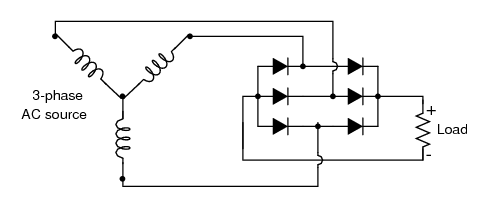
\includegraphics[scale=0.4]{ucfaz}
\caption{Rectifier Topology}
\label{fig:members}
\end{figure}

These changes on conduction determine output voltage waveform. The output waveform operation can be seen from following figure 12. Because the output value of the rectifier is higher than our expected output. We have connected a buck converter to arrange output voltage level. The buck converter operation will be covered at following section.
\begin{figure}[h!]
\centering
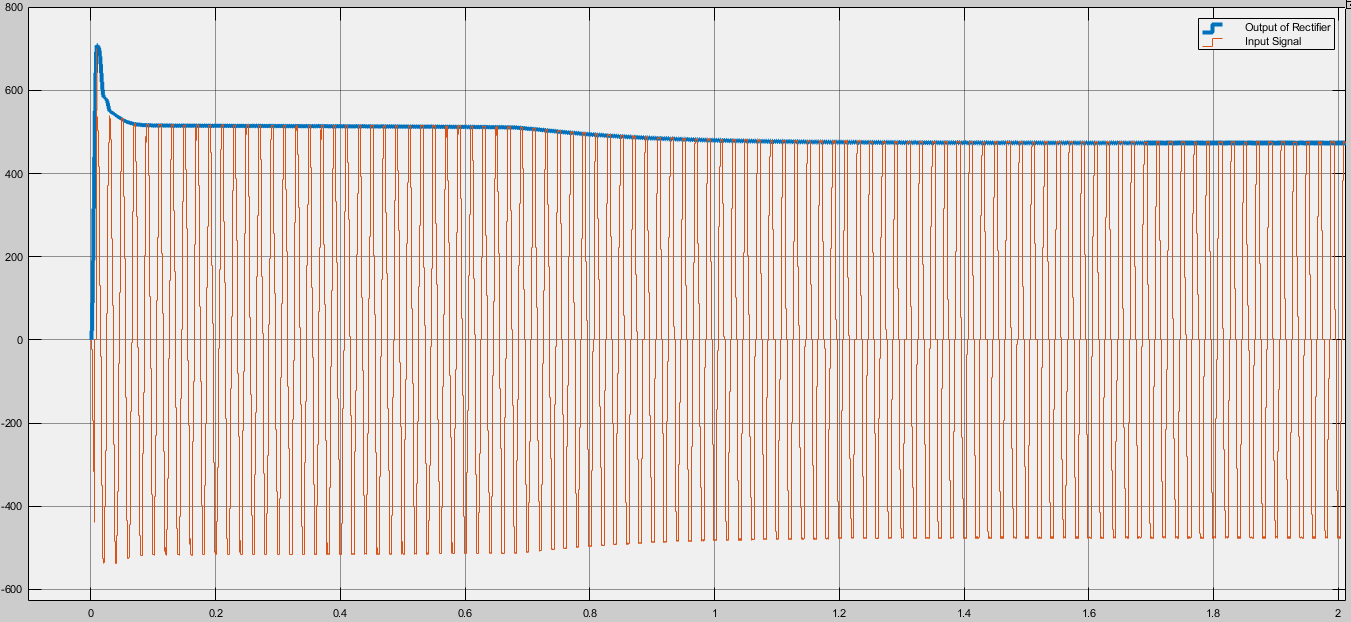
\includegraphics[scale=0.25]{ucfazrectvoltage}
\caption{Rectifier Operation}
\label{fig:members}
\end{figure}


\subsection{Buck Converter}

The reason of using buck converter in our circuit, which is shown in figure 13 is setting the output voltage to a optimum level by controlling the switching of the IGBT.
\begin{figure}[H]
\centering
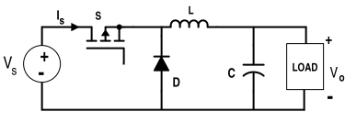
\includegraphics[scale=0.7]{bucktopo}
\caption{Buck Converter Topology}
\label{fig:members}
\end{figure} 

\par The buck converter's working principle bases on duty cycle of the switching waveform of gate signal. During switch is ON period, the diode goes OFF and we charge our inductor. After then, we discharge our inductor on load and diode during switch is OFF period. The simulation result is indicated at following figure;

\begin{figure}[H]
\centering
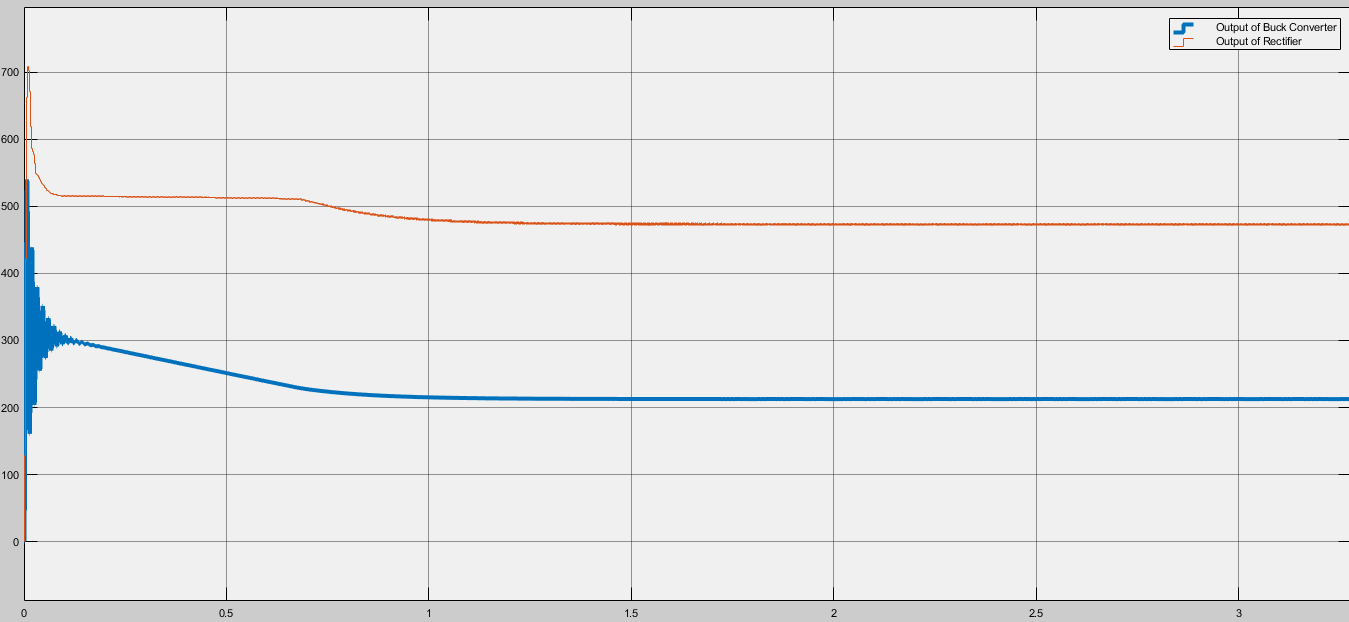
\includegraphics[scale=0.25]{buckvoltage}
\caption{Buck Converter Operation}
\label{fig:members}
\end{figure}

\subsection{Overall System Results}
After obtaining the operations of each subunit; we combined them as an overall system which can be seen from figure 15. The following figures indicates the input output relations of the circuit for different conditions; 

\begin{figure}[H]
\centering
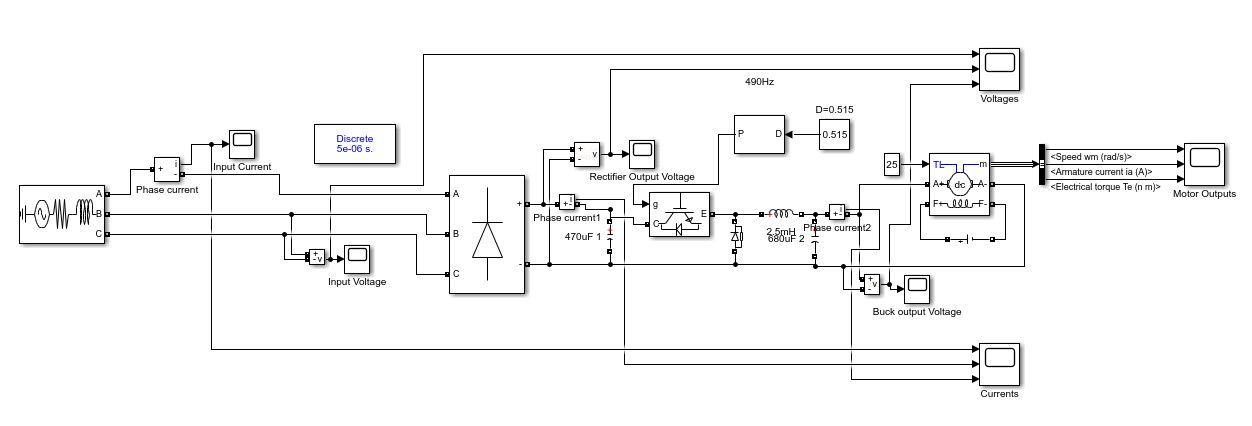
\includegraphics[scale=0.45]{ucfazdiyotbuck}
\caption{Overall Circuit}
\label{fig:members}
\end{figure}

\begin{figure}[H]
\centering
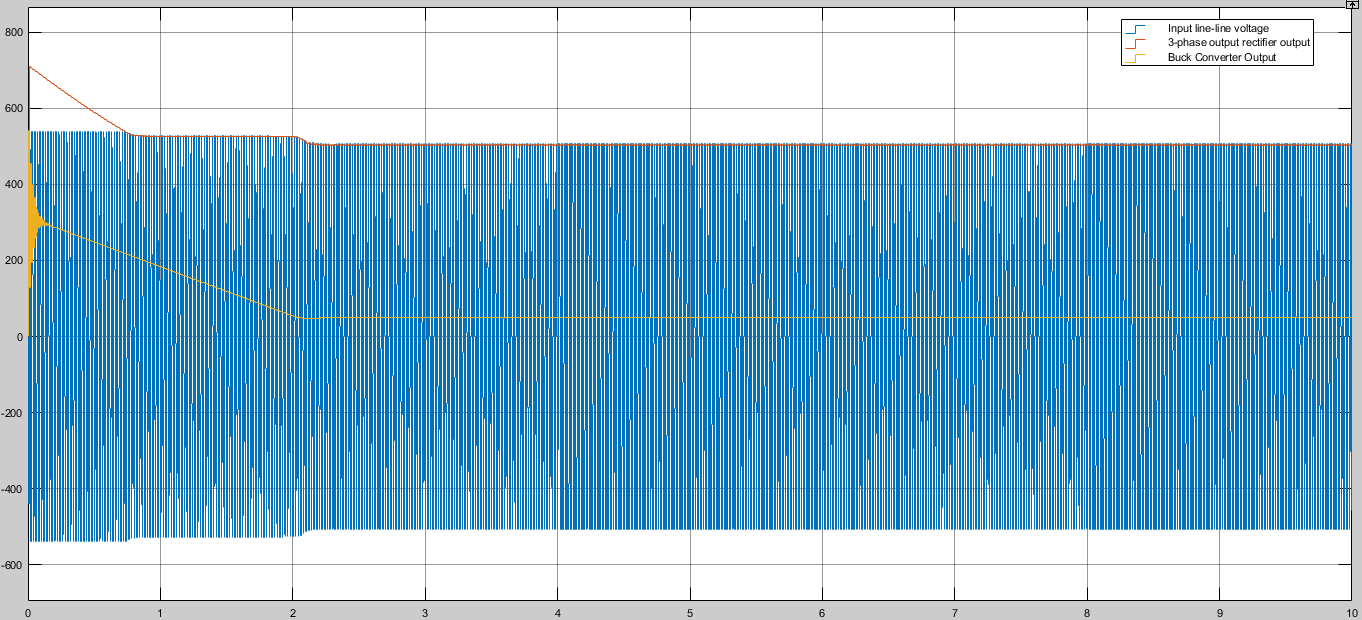
\includegraphics[scale=0.25]{voltagesnoktaonduty}
\caption{\% 10 Duty Cycle Voltage Output}
\label{fig:members}
\end{figure}

\begin{figure}[H]
\centering
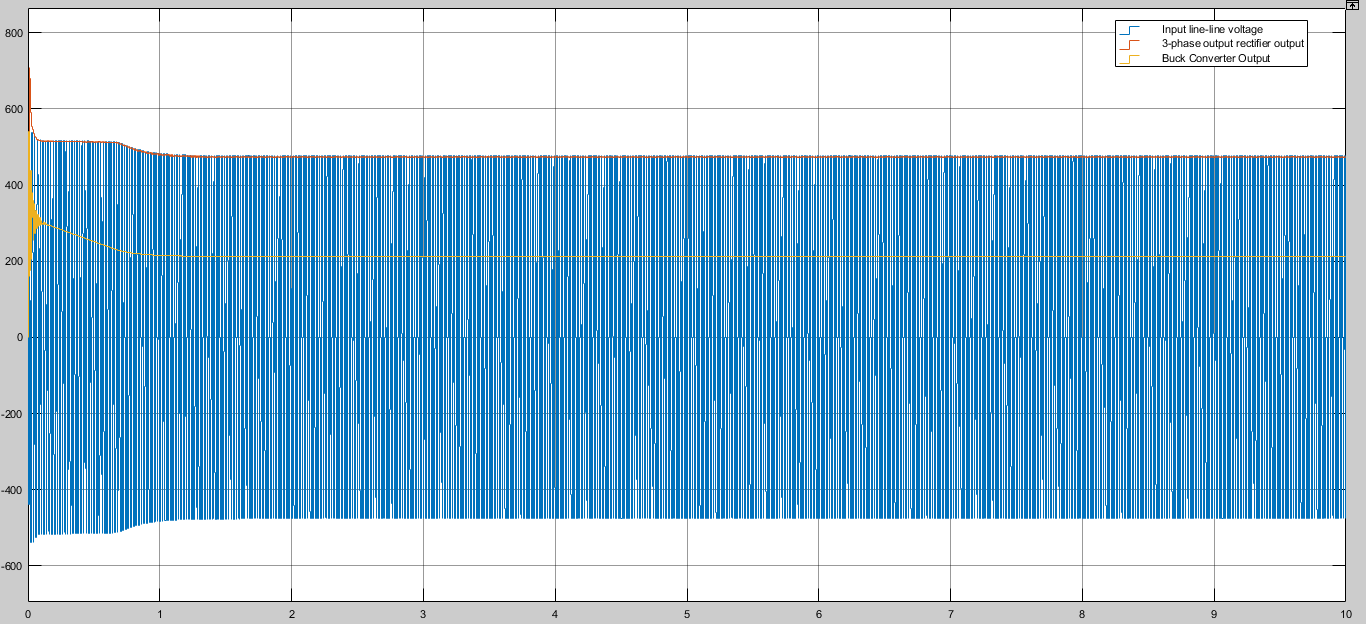
\includegraphics[scale=0.25]{voltagesnoktabesduty}
\caption{\% 50 Duty Cycle Voltage Output}
\label{fig:members}
\end{figure}

\begin{figure}[H]
\centering
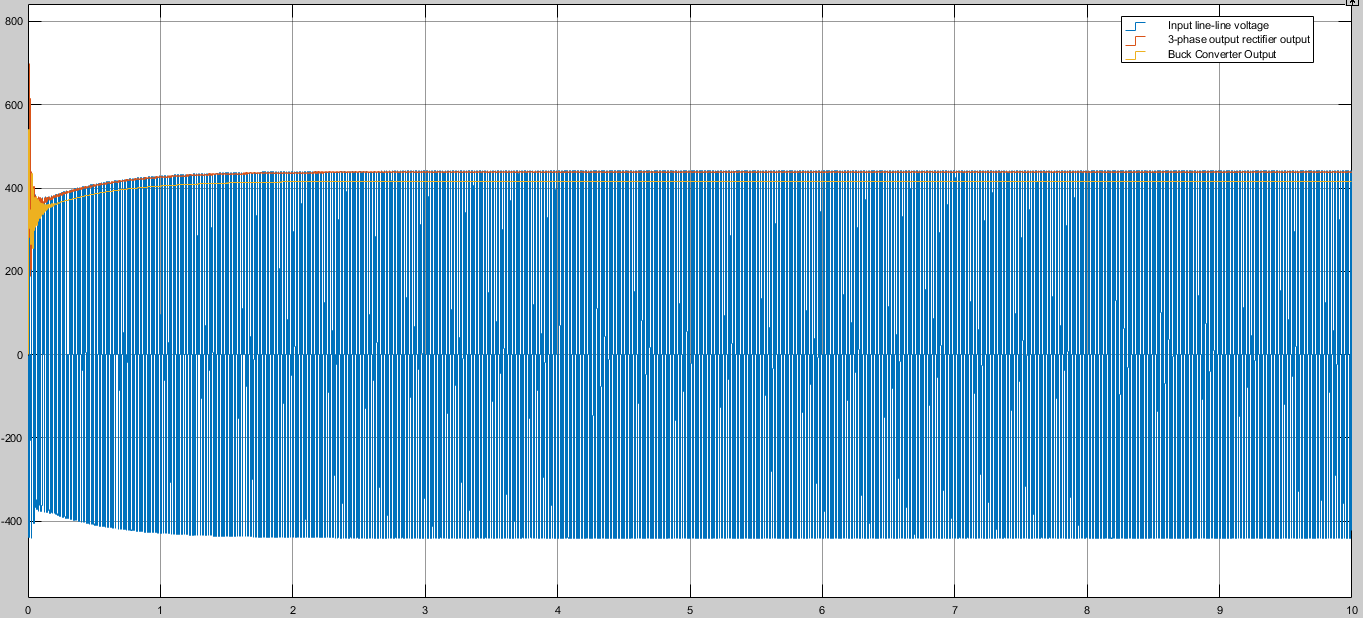
\includegraphics[scale=0.25]{voltagesnoktadokuzduty}
\caption{\% 95 Duty Cycle Voltage Output}
\label{fig:members}
\end{figure}

\begin{figure}[H]
\centering
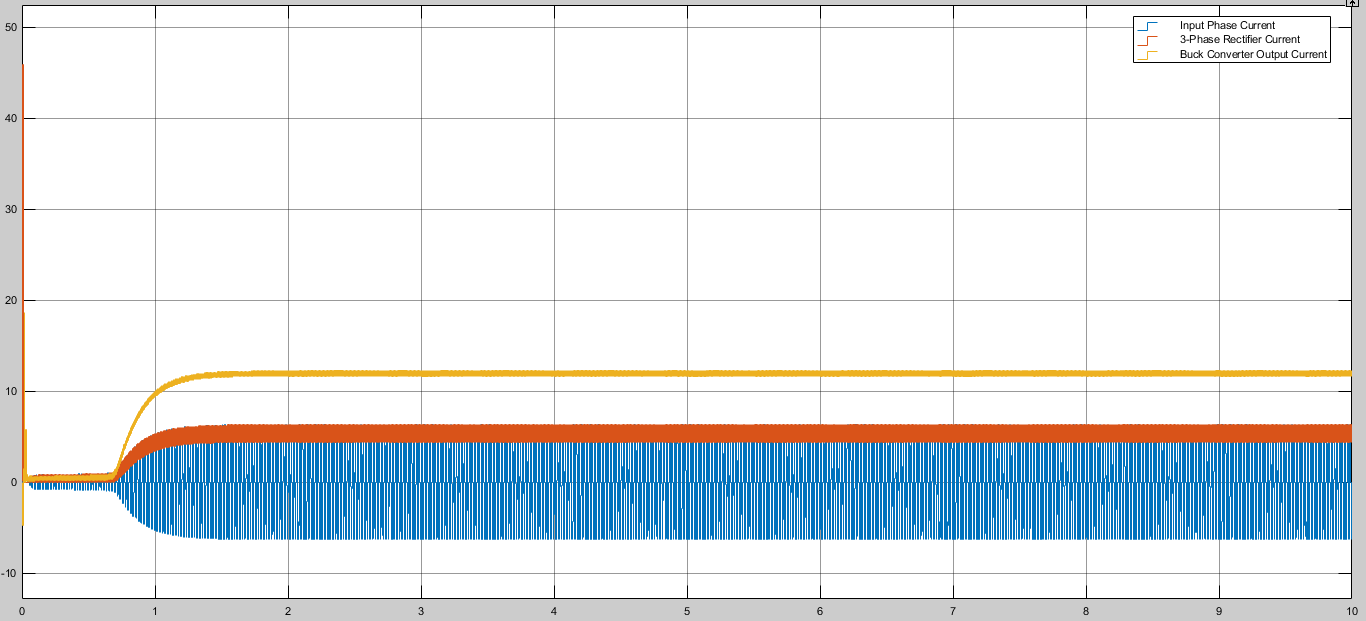
\includegraphics[scale=0.25]{diodebuckcurrents}
\caption{Current Analysis of Simulation Circuit for \% 50 Duty Cycle }
\label{fig:members}
\end{figure}

\begin{figure}[H]
\centering
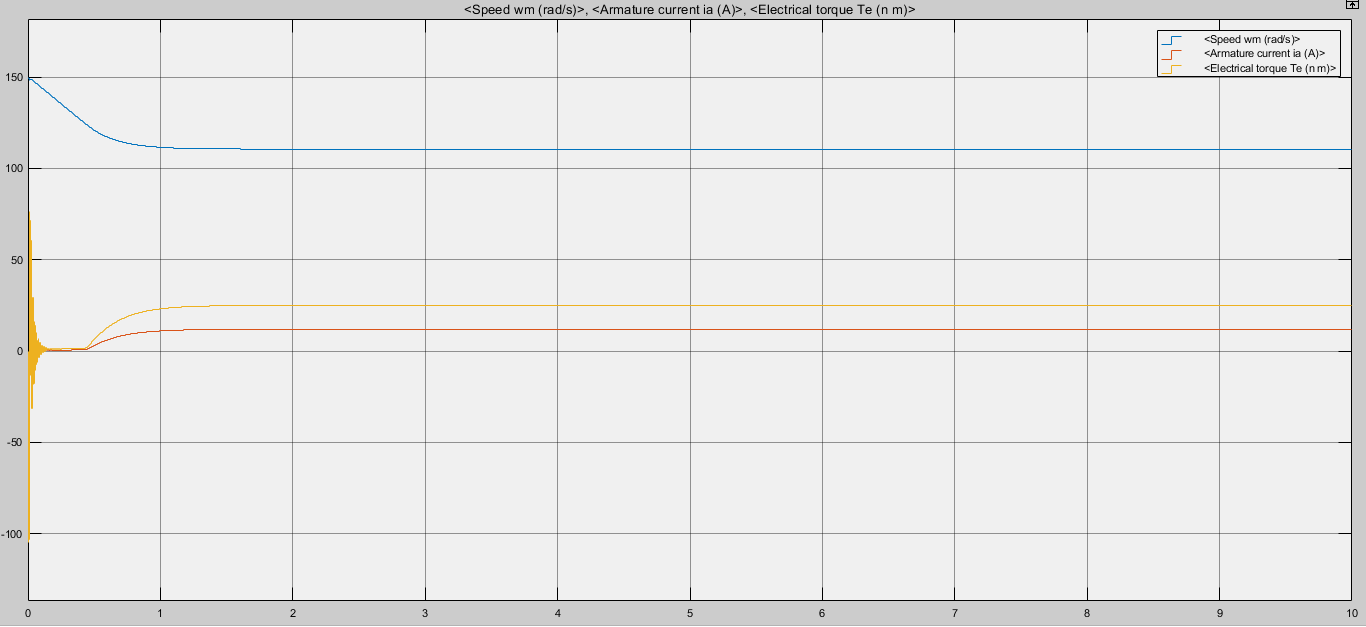
\includegraphics[scale=0.25]{torkvs}
\caption{Speed-Armature Current-Electrical Torque vs Time Graph }
\label{fig:members}
\end{figure}



\section{Component Selection}
According to the simulation results we have determined to get components indicated at table 3. While buying the components we were flexible about parameters, because some components are hard to find in local shops. 

\noindent Table 3: Component List
\begin{figure}[H]
\centering
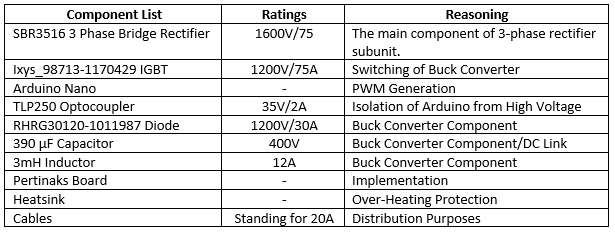
\includegraphics[scale=0.8]{componentselection}
\label{fig:members}
\end{figure} 

\textit{*For more detailed information, please see our Github repository's datasheets section.}

\section{Test Results}%Samet
After component selections; we implemented the circuit on board(can be seen from figure 21) and applied some tests. As seen in figure 22; when output voltage of full bridge rectifier is 232 V; Duty Cycle, Collector to Emitter Voltage and Output Voltage is given in figure 23. 

\begin{figure}[H]
\centering
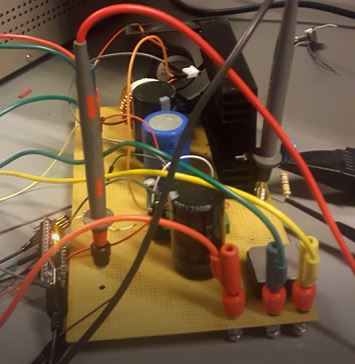
\includegraphics[scale=0.6]{devre}
\caption{The product during test process }
\label{fig:members}
\end{figure}


\begin{figure}[H]
\centering
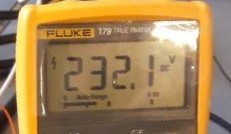
\includegraphics[scale=0.7]{testoutput}
\caption{The Measured Output Voltage at Rectifier}
\label{fig:members}
\end{figure}

\begin{figure}[H]
\centering
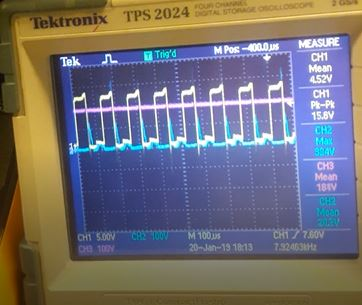
\includegraphics[scale=0.6]{testone}
\caption{The Output Voltage Waveforms }
\label{fig:members}
\end{figure}

\section{Demonstration Results}%Samet
At the final day of the project, we presented our project to the expert. The product is worked well and managed to complete some task such as full loaded working for a while. The following figures show outputs taken during demonstration. 
\begin{figure}[H]
\centering
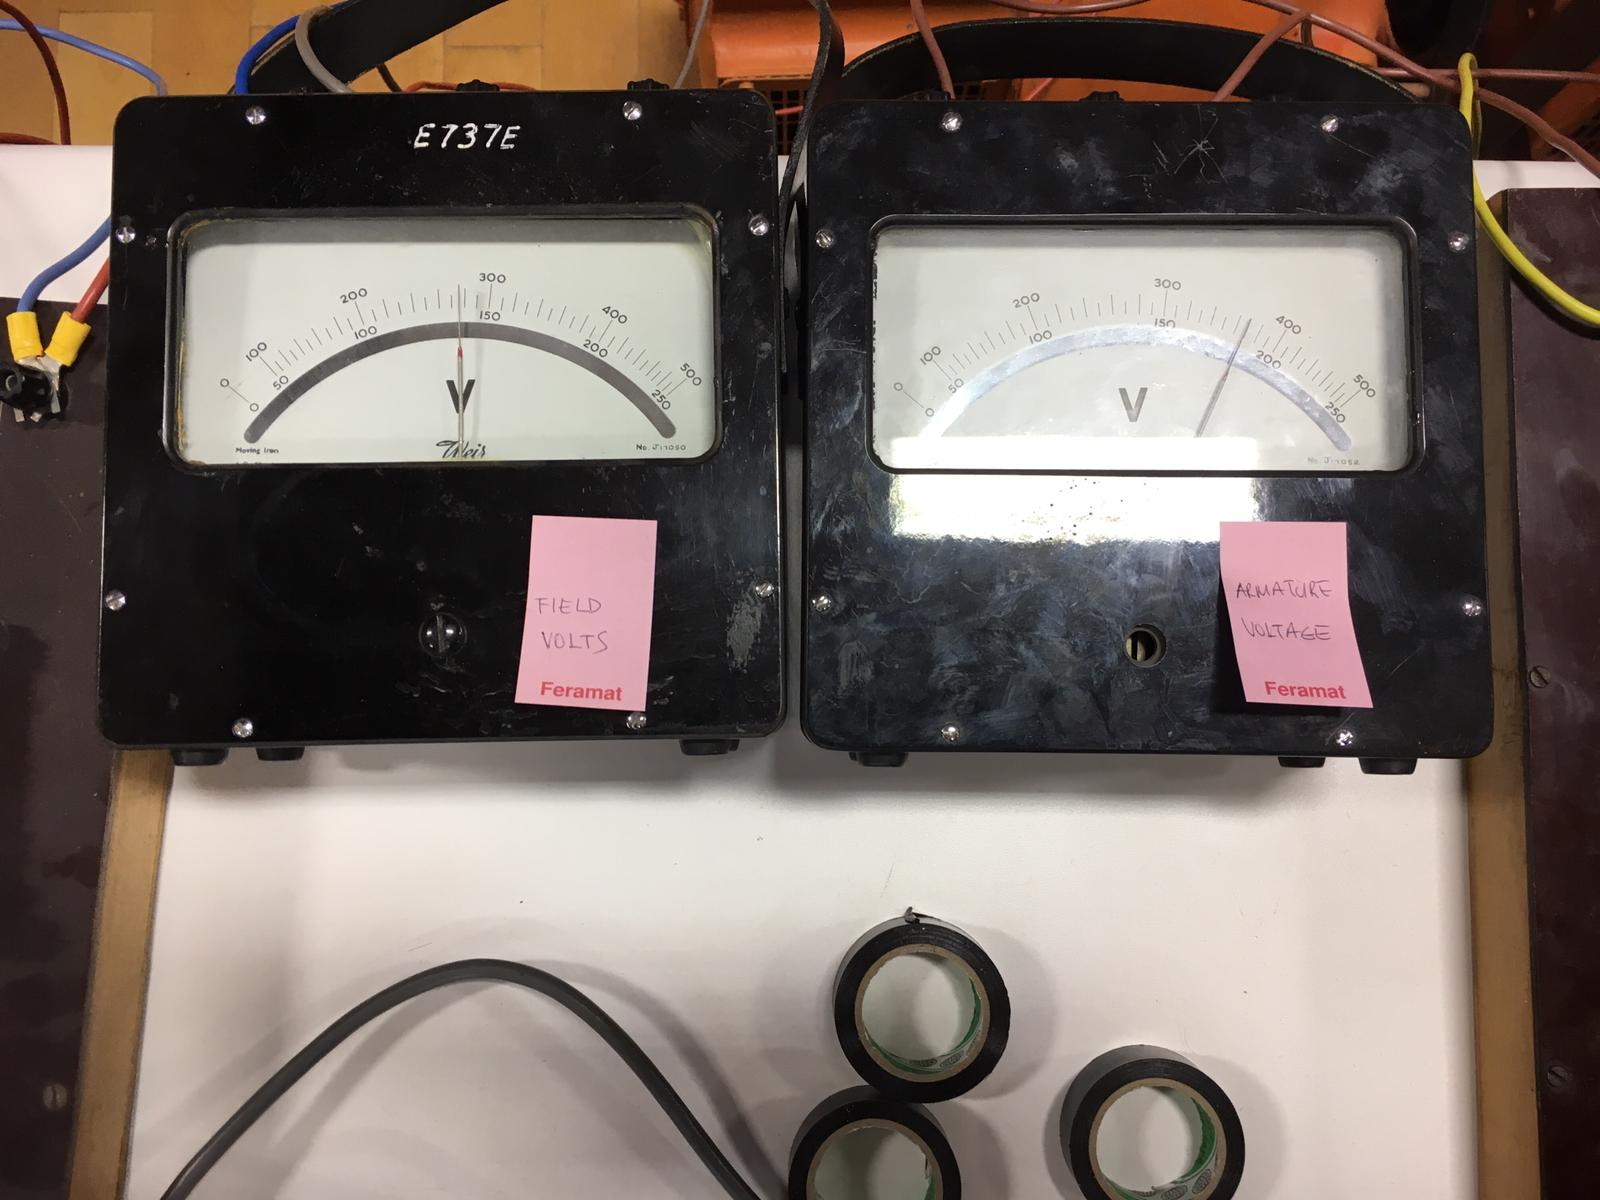
\includegraphics[scale=0.1]{demofield.jpg}
\caption{Field and Armature Voltage at Full Load}
\label{fig:members}
\end{figure}

\begin{figure}[H]
\centering
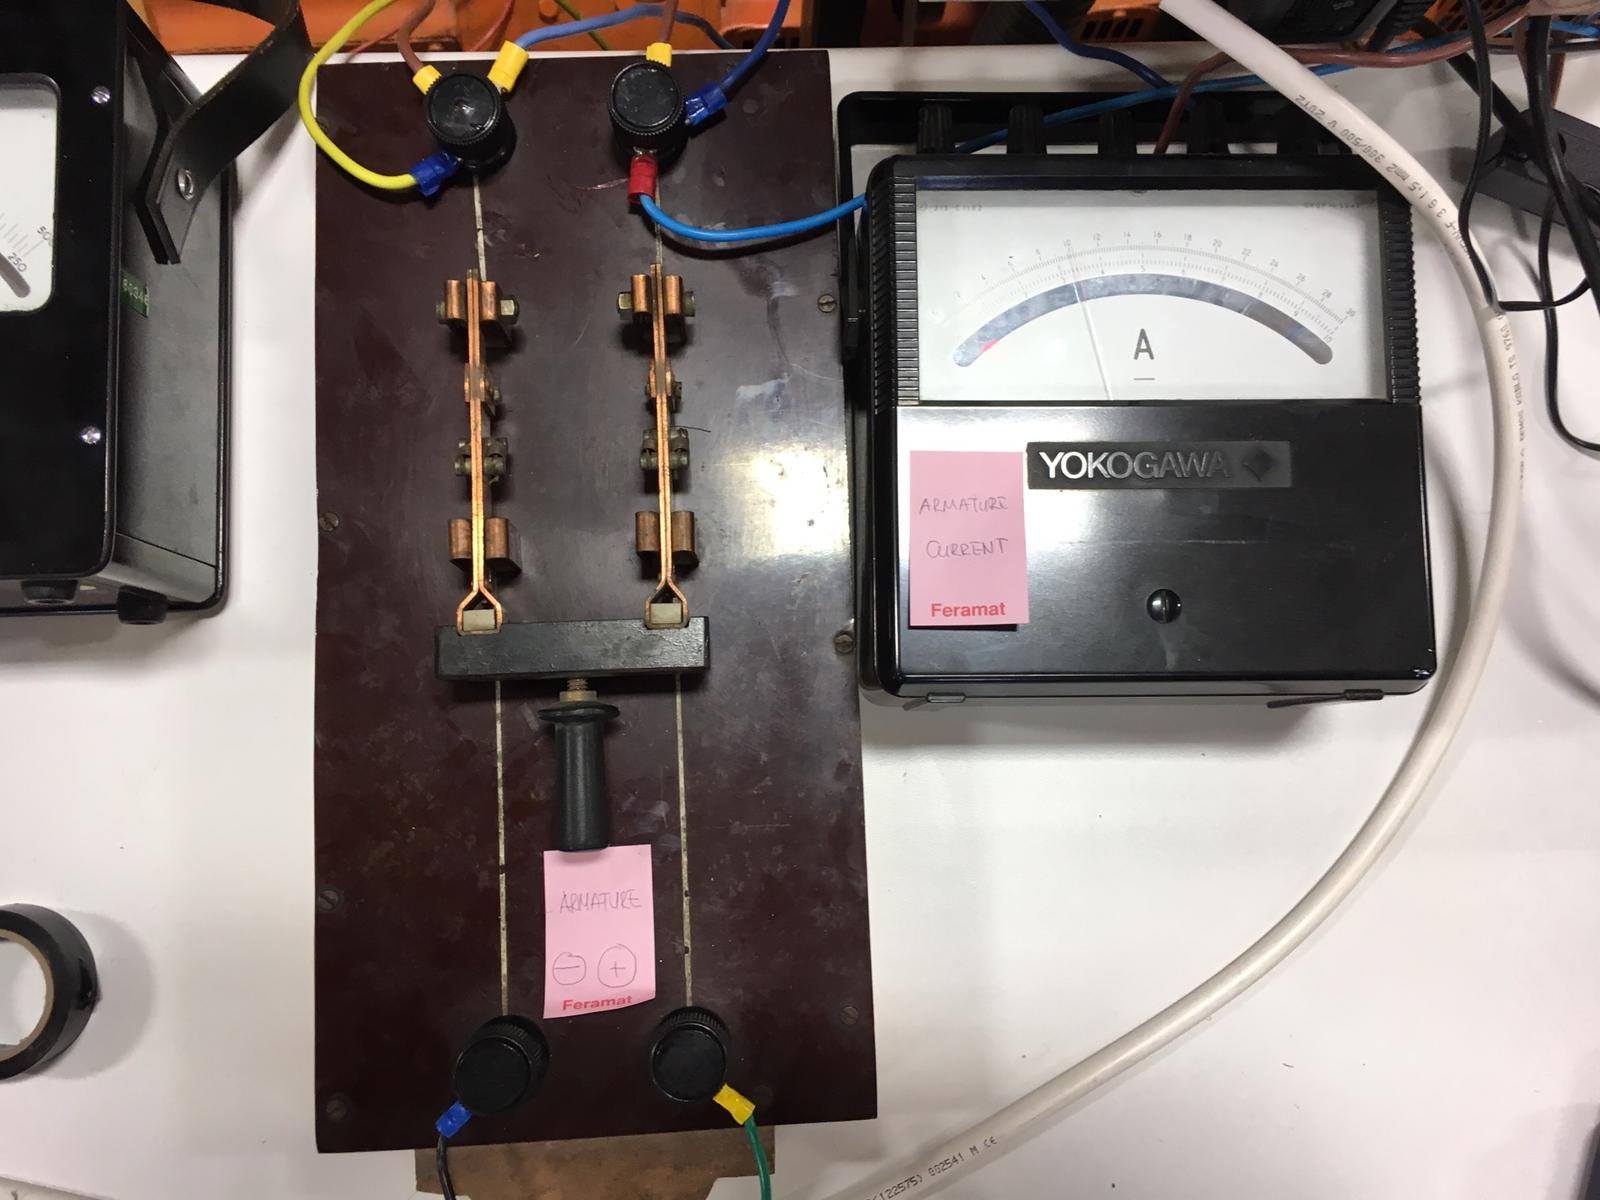
\includegraphics[scale=0.1]{demoarmaturecurrent}
\caption{Armature Current at Full Load Condition  }
\label{fig:members}
\end{figure}

\begin{figure}[H]
\centering
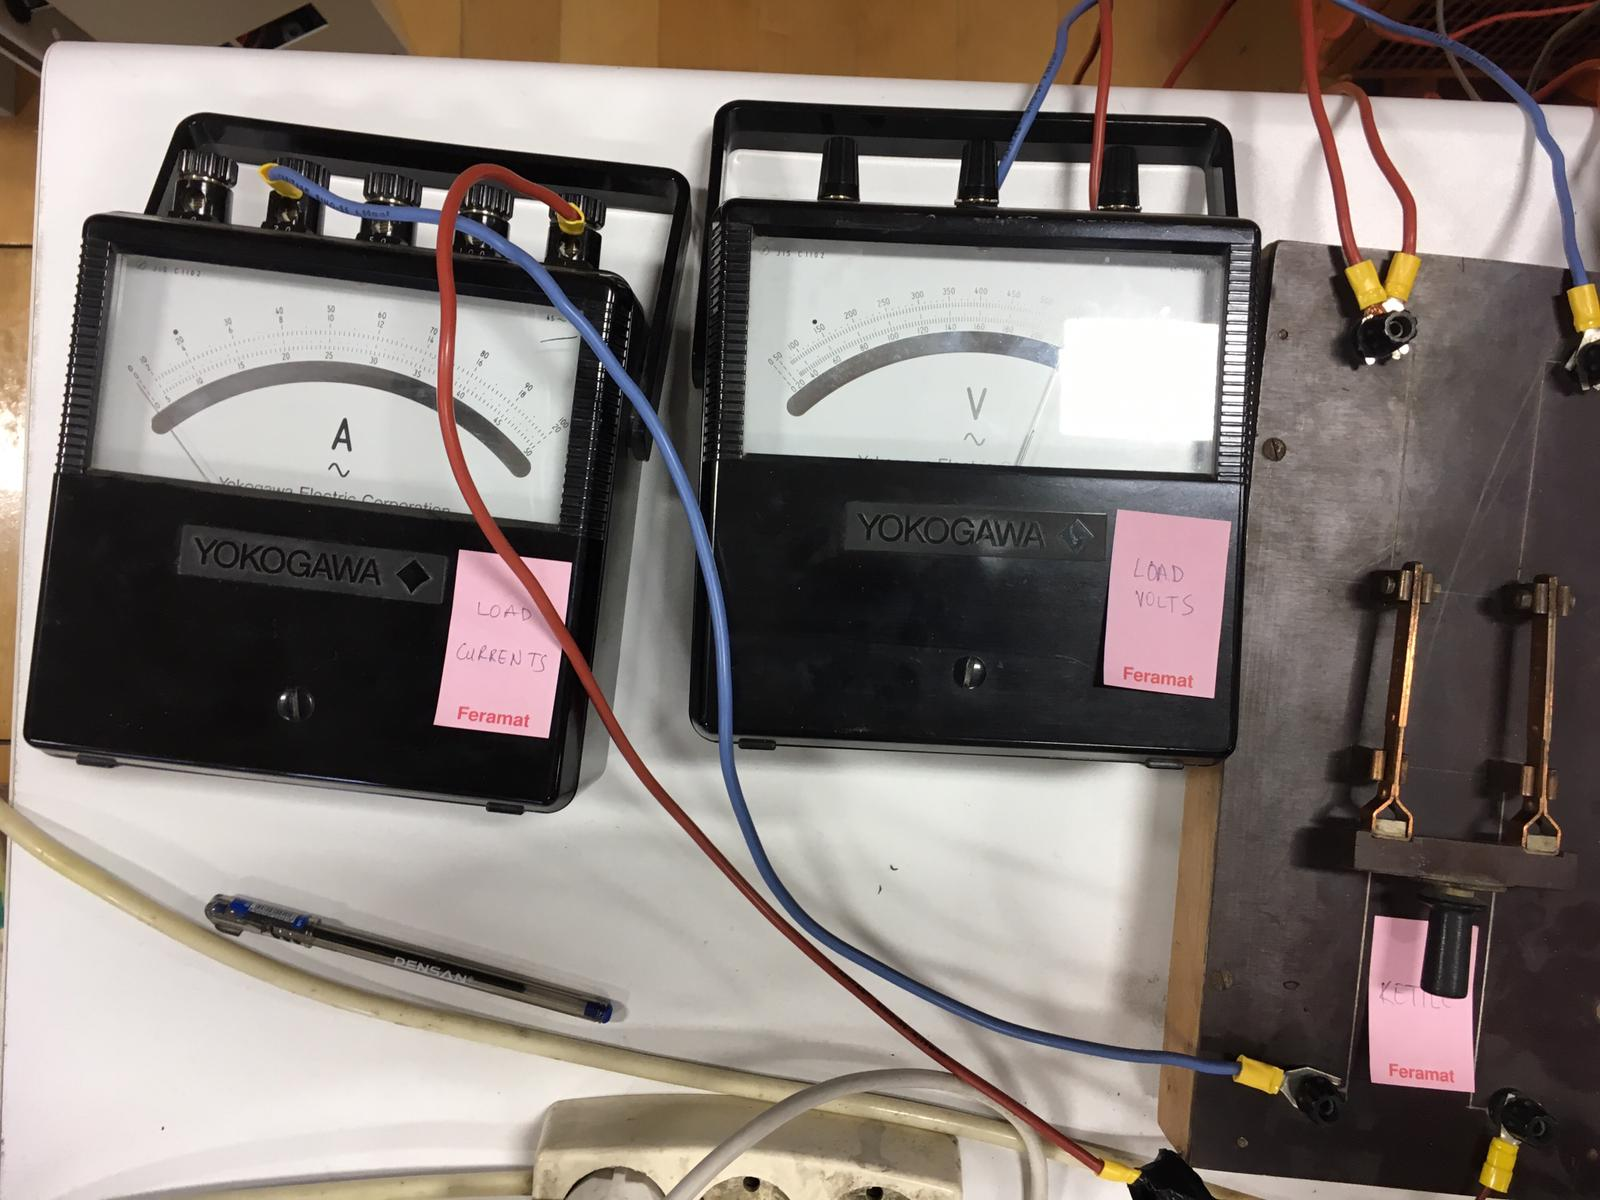
\includegraphics[scale=0.1]{demovoltagecurrent2.jpg}
\caption{Load Voltage and Load Current}
\label{fig:members}
\end{figure}

\begin{figure}[H]
\centering
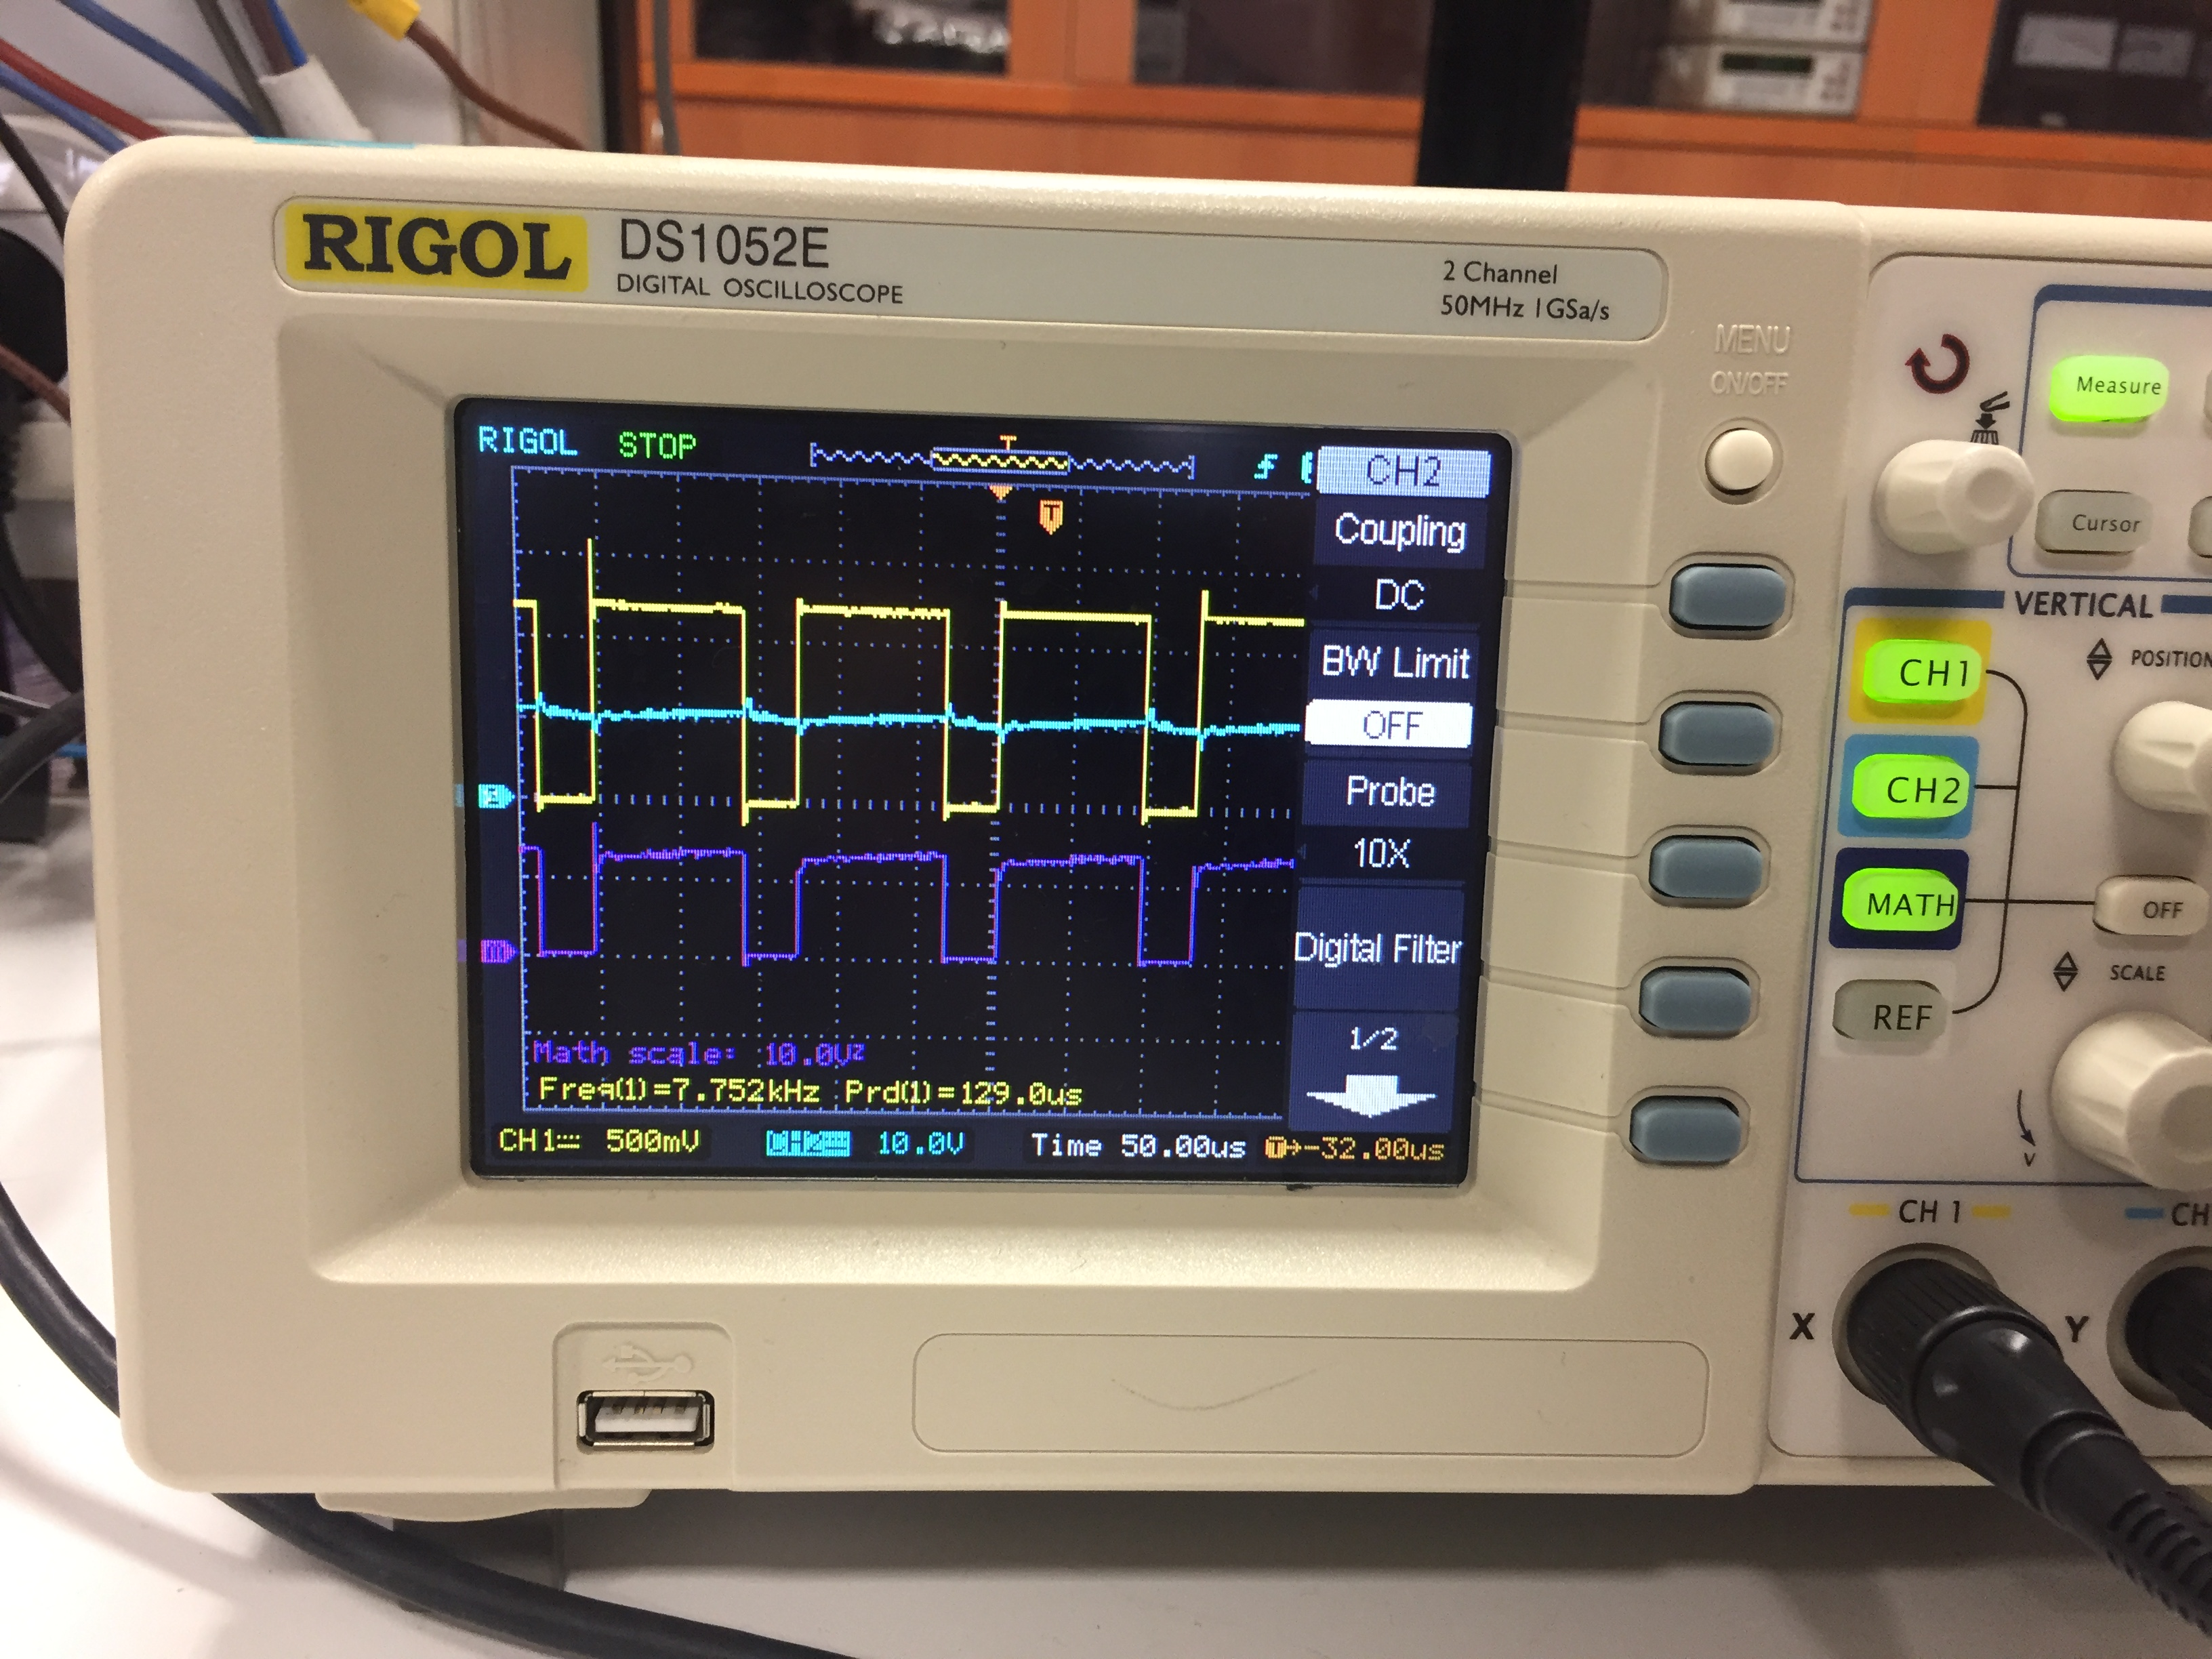
\includegraphics[scale=0.05]{demovoltagecurrent}
\caption{Load Voltage, Current and Power Waveforms }
\label{fig:members}
\end{figure}

\section{Cost Analysis}
During test process, we have faced lots of problems as expected. Fortunately, we had spare components in order to replace with damaged ones. For example, because of overshoots at \(V_{CE}\) voltage, we burnt 4 IGBTs. In addition, we burnt one diode because of high switching frequency. The other problem that we faced is because of a unexpected short circuit, the TLP250 is burnt. Therefore, all these failures became good experiences for us. The finalized version of cost analysis can be seen from following table;

\noindent Table 4: Cost Analysis
\begin{figure}[H]
\centering
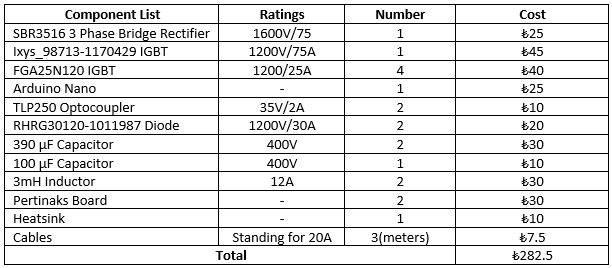
\includegraphics[scale=0.9]{cost}
\label{fig:members}
\end{figure} 

\newpage
\section{Conclusion}
We are asked to produce an AC to DC Motor Driver in order to drive a specified DC motor under full load. The speed of the motor also should be controlled by hand. In demonstration, the project is successfully delivered by qualified engineers of FOSFOS Actiengesellschaft.
\par During this process, we divided our project into subunits to increase ease of understanding concepts. After understanding the project clearly, we went MATLAB/Simulink environment and simulated our design. According to the design, the components of the product is determined. The most challenging part of the project was implementation and testing processes. We have faced too many problems during that period because simulation world is all ideal. The one and most important issue that we faced during testing is over-heating problem. Because we did not use thermal paste between IGBT and heatsink, we lost 4 IGBT's. The other problem was in simulations that the snubber values of the IGBT is set to be ideal, but in real life it is not. Because of inductive effects in cables, we could not handle this problem at first and lost some IGBTs due to overshooting at voltage. The last problem that we faced is parasitic elements caused some problems. After then, we learned that a practical solution which can solve this problem. By connecting a little capacitor between collector of IGBT and anode of the diode, problems could be solved.

\par Although project is tiring and hard to create, we learned too many things to use our future engineering life. This project is also helped us to understand the consepts of EE463 Static Power Conversion Course. Finally we would like to thank our Instructors, power elctronics M.S. Students and laboratory technician for their helps.

\section{References}
MOHAN, N. (2017). Power Electronics JOHN WILEY \& Sons.\\
http://keysan.me/ee463/  \\
https://github.com/sametyildirima/FosFos-AG.git\\
http://www.seklad69associates.com/seklad69associates.com/EEG\_811\_files/Semiconductor\%20Physics.pdf



\section*{Appendices}
\textbf{Arduino Code for PWM Generation} 
\begin{figure}[H]
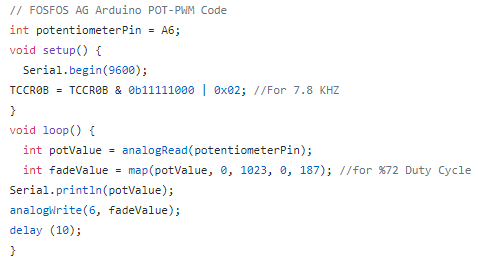
\includegraphics[scale=0.8]{pwmcode}
\label{fig:members}
\end{figure} 
\noindent \textbf{Datasheets} \\
https://github.com/sametyildirima/FosFos-AG/blob/master/Datasheets/2282907.pdf\\
https://github.com/sametyildirima/FosFos-AG/blob/master/Datasheets/2822\_7668536.pdf\\
https://github.com/sametyildirima/FosFos-AG/blob/master/Datasheets/FGA25N120.pdf\\
https://github.com/sametyildirima/FosFos-AG/blob/master/Datasheets/FGH20N60SFD-D.PDF\\
https://github.com/sametyildirima/FosFos-AG/blob/master/Datasheets/RHRG30120-1011987.pdf\\
https://github.com/sametyildirima/FosFos-AG/blob/master/Datasheets/TLP250(INV)\_datasheet\_en\_20170821.pdf\\
https://github.com/sametyildirima/FosFos-AG/blob/master/Datasheets/ixys\_98713-1170429.pdf\\
\noindent \textbf{Video Link(In Turkish)} \\%Samet\\
https://www.youtube.com/watch?v=irYZJVu4fXo&feature=youtu.be
\end{document}
